\documentclass{llncs}

\usepackage[spanish]{babel}
\usepackage{makeidx}
\usepackage{graphicx}

\begin{document}

\mainmatter

\title{ MediCub: \textit{un asistente médico impulsado por IA} }
\titlerunning { MediCub }

\author{Darío López Falcón\inst{1} \and Eduardo Brito Labrada\inst{1} \and Ernesto Abreu Peraza\inst{1}}
\authorrunning{Darío López Falcón \and Eduardo Brito Labrada \and Ernesto Abreu Peraza}

\institute{Facultad de Matemática y Computación, Universidad de La Habana}

\maketitle

\begin{abstract}

MediCub\footnote{\url{https://github.com/ArcanoxXx-01/MediCub}} es un asistente médico basado en inteligencia artificial diseñado para apoyar a médicos durantes consultas o servir
como herramienta de preconsulta para pacientes. El sistema simula el razonamiento clínico humano mediante etapas que incluyen
la extracción de entidades médicas, generación de posibles diagnósticos, retroalimentación iterativa y recomendación basadas en
pruebas.
\keywords{inteligencia artificial, simulación, sistemas de recuperación de la información, salud}
\end{abstract}

\section{Introducción}

Es muy común en muchos hospitales, que los pacientes tengan que enfrentarse a largos tiempo de espera o incertidumbre sobre la urgencia o gravedad de sus síntomas. Esta
situación no solo incrementa la carga de trabajo para los profesionales de la salud, sino que también puede retrasar diagnósticos cruciales y afectar la calidad de la atención
médica.

Ante esta problemática, nace MediCub, un asistente médico impulsado por inteligencia artificial, diseñado con el objetivo de brindar apoyo durante las consultas clínicas y 
funcionar como una herramienta de preconsulta para los pacientes. El sistema se enfoca en interpretar consultas escritas en lenguaje natural, analizando síntomas, antecedentes 
médicos y dolencias reportadas por el paciente, para luego generar un prediagnóstico razonado y estructurado.

A diferencia de otros sistemas existentes, MediCub no se limita a listar posibles enfermedades, sino que simula el razonamiento de un médico humano, siguiendo un proceso iterativo
de análisis, inferencia y retroalimentación con el paciente; su funcionalidad se extiende para identificar entidades médicas relevantes (síntomas, enfermedades, tratamientos), propone
posibles diagnósticos y realiza preguntas adicionales para refinar su comprensión del caso.

Es importante destacar que MediCub no pretende sustituir al profesional de la salud, sino complementar su labor, facilitando la recolección inicial de información clínica y ofreciendo 
una visión preliminar del caso. Con ello, se busca mejorar la eficiencia del proceso diagnóstico, optimizar el tiempo del personal médico y fortalecer el acceso a una atención más oportuna
y personalizada.

\section{Solución}

La solución propuesta se basa en la simulación computacional del comportamiento de un médico humano durante una consulta clínica. El procedimiento se divide en varias etapas que permiten el correcto
funcionamiento de esta solución:

\begin{enumerate}
  \item \textbf{Explicación inicial del paciente}: Esta etapa inicia con una consulta en lenguaje natural, en la que el paciente describe su situación médica: síntomas, antecedentes, molestias o eventos recientes
  que le hayan sucedido y que considere importante. Esto constituye la base fundamental para las siguientes etapas.
  \item \textbf{Extracción de entidades médicas}: El sistema emplea técnicas de procesamiento de lenguaje natural para identificar y extraer las entidades médicas relevantes del texto ingresado por 
  el paciente, esas entidades incluyen síntomas, enfermedades conocidas, tratamientos previos, factores de riesgo, etc.
  \item \textbf{Descarte por conocimiento médico}: Utilizando una base de conocimiento clínico estructurada, el sistema asocia las entidades extraídas con un conjunto preliminar de enfermedades compatibles (conjunto $E_1$).
  Esta inferencia se basa en correlaciones semánticas y relaciones clínicas entre síntomas y patologías.
  \item \textbf{Retroalimentación y acotamiento del diagnóstico}: Si la información inicial no permite determinar un diagnóstico probable, el sistema genera preguntas adicionales orientadas a reducir la ambigüedad diagnóstica.
  Estas preguntas son seleccionadas de forma estratégica para maximizar la discriminación entre posibles enfermedades, priorizando síntomas clave.
  \item \textbf{Etapa de iteración}: Las respuestas del paciente alimentan una nueva ronda de inferencia, actualizando el conjunto de enfermedades probables. Este ciclo de retroalimentación continúa hasta alcanzar un conjunto
  reducido de hipótesis diagnósticas con alta probabilidad.
  \item \textbf{Descartes por pruebas}: En una etapa posterior, se simula el razonamiento médico basado en pruebas clínicas. Aunque el sistema no puede ordenar la realización de pruebas o estudios, puede sugerir realizar pruebas
  que resultados hipotéticos confirmarían o descartarían una enfermedad específica.
  \item \textbf{Prediagnóstico}: Finalmente, el sistema presenta un resumen con el conjunto de enfermedades más probables, junto con las entidades detectadas, las relaciones inferidas y la justificación clínica correspondiente.
  Este resultado se entrega como una ayuda al profesional médico o como orientación preliminar al paciente.
\end{enumerate}

Además de este diseño basado en etapas, que permite el correcto funcionamiento del sistema, se tomaron en cuenta varias consideraciones técnicas, éticas y prácticas. En primer lugar, se definió que este sistema solo actuaría como un
asistente médico y no como sustituto de un profesional de la salud, por lo que sus funcionalidades están limitadas a brindar una orientación preliminar. Se priorizó el uso de esta herramienta para hispanohablantes, por lo que se utilizaron
fuentes confiables y accesibles en español, como MedlinePlus\cite{medlineplus}, para garantizar que la información médica se mantenga actualizada se diseñaron componentes como el crawler y un actualizador de la base de datos. Se tuvo en cuenta
que este sistema no solo iba a ser utilizado por usuarios con formación técnica, por lo que se utilizó una interfaz clara y comprensible así como el procesamiento de lenguaje natural. En términos de interacción, se adoptó un enfoque conversacional
empático con preguntas claras simulando el razonamiento de un médico.

Para validar las respuestas dadas por el sistema se utilizaron tanto consultas manuales, que permitieron tener retroalimentación más directa de qué tan cómodo iba a ser para el usuario interactuar con el sistema; y se utilizaron pruebas automáticas
extraídas de Fisterra\cite{fisterra}.

\subsection{Componentes principales utilizadas}

A partir de la descomposición funcional del razonamiento médico simulado, se definieron componentes esenciales para que el sistema pudiera ejecutar dicha simulación de forma efectiva y estructurada:

\begin{itemize}
  \item \textbf{Orquestador}: esta es la componente fundamental del sistema ya que coordina la interacción entre los distintos componentes del mismo, en cada momento decide que módulo debe activarse en dependencia del estado actual de la información extraída hasta el momento. Se diseñó
  con una arquitectura modular que integra varios componentes claves del sistema. A continuación se describe el funcionamiento de esta componente.
  \begin{enumerate}
    \item \textbf{Procesador de consultas}: Esta componente tiene como objetivo normalizar el texto de entrada y extraer la información médica relevante a partir de una consulta escrita en lenguaje natural. Para ello, realiza tareas de preprocesamiento como la ``limpieza" del texto y la
    extracción de entidades médicas tales como síntomas, enfermedades o antecedentes mencionados por el usuario.
    \item \textbf{Generación de embeddings}: Las entidades extraídas fueron transformadas en vectores mediante un modelo de embeddings semánticos, lo cual permite medir similitud con la base vectorial.
    \item \textbf{Búsqueda Semántica en la Base Vectorial}: Se compararon los vectores de entrada con los vectores prealmacenados de documentos médicos procesados previamente (chunks). Se realizó un ranking de resultados basado en la similitud.
    \item \textbf{Selección de resultados relevantes}:  Se conservaron únicamente los $k$ documentos con mayor similitud que superaban un umbral predefinido. Estos documentos aportaron información útil adicional para enriquecer el diagnóstico.
    \item \textbf{Diagnóstico Inicial}: Se generó un diagnóstico preliminar utilizando solo las entidades extraídas de la consulta original.
    \item \textbf{Evaluación de Entidades Recuperadas}:  Se evalua si alguna de las entidades médicas adicionales encontradas en los documentos recuperados tenía potencial para mejorar el diagnóstico. Si se identificaba alguna, esta se presentaba al usuario como una pregunta de seguimiento.
    \item \textbf{Interacción con el usuario}: Se consulta al usuario si presentaba dicha entidad. En caso afirmativo, se repitió el paso de diagnóstico incluyendo esta nueva información.
    \item \textbf{Repetición hasta convergencia}: El ciclo diagnóstico-pregunta se repitió hasta que el sistema alcanzaba un umbral de confianza en el diagnóstico, no se identificaban más entidades con ganancia diagnóstica relevante o el usuario rechazaba todas las entidades adicionales.
    \item \textbf{Generación de Respuesta Final}: Se genera una respuesta empática y clara para el usuario final, explicando el diagnóstico más probable y los motivos médicos subyacentes, utilizando un modelo LLM y un prompt especializado.
    \item \textbf{Tolerancia a Fallos}: En cualquier etapa donde se produjera un error, el orquestador continuaba con el mejor resultado disponible hasta el momento, garantizando que el usuario recibiera siempre una respuesta funcional.
  \end{enumerate}
  \item \textbf{Expansor de consulta}: Este componente abarca varias etapas de razonamiento clínico automatizado y se encarga de enriquecer e interpretar la información extraída. Está compuesto por una base de metadatos vinculada a vectores indexados, un
  generador de rankings que ordena posibles diagnósticos, un generador de preguntas para refinar la información provista por el usuario y una fase de retroalimentación que permite iterar sobre nuevas respuestas para mejorar la precisión del prediagnóstico.
  \item \textbf{Crawler y actualizador de la base de datos}: Este agente automatizado tiene como función mantener actualizada la base documental médica del sistema, la cual se nutre principalmente de MedlinePlus\cite{medlineplus} en español. Este módulo está compuesto
  por varios submódulos:
  \begin{itemize}
    \item Un scraper de artículos, que obtiene el código HTML de nuevos documentos o de aquellos cuya última descarga es obsoleta.
    \item Un extractor de información, encargado de procesar dicho HTML para identificar elementos claves como causas, síntomas, nombres alternativos, procedimientos a realizar y contraindicaciones.
    \item Un chunker, que divide la información extraída en fragmentos o ``chunks", cada uno acompañado de su correspondiente metadato.
    \item Un modelo de embedding que genera vectores representativos de cada chunk para su posterior indexación y recuperación. En este trabajo, debido a limitaciones de recursos, se utilizó un modelo gratuito ofrecido por Fireworks\cite{fireworks_ai}
  \end{itemize}
  \item \textbf{Medical graph builder}: es el componente encargado de representar y explotar conocimiento médico estructurado en forma de un grafo dirigido. Su inclusión dentro del sistema de diagnóstico tuvo como finalidad complementar los resultados derivados del procesamiento semántico 
  (embeddings) con inferencias explícitas basadas en relaciones conocidas entre enfermedades, síntomas y causas. Su objetivo principal es representar el conocimiento médico como un grafo dirigido, donde los nodos son entidades clínias y las aristas representan relaciones relevantes (por ejemplo, ``causa de", ``síntoma de", etc.),
  esto proporciona operaciones de consultas como: encontrar entidades relaciones, sugerir posibles diagnósticos asociados a síntomas y explorar caminos diagnósticos alternativos.
  El grafo fue implementado mediante \texttt{networkx.DiGraph}.
\end{itemize}

\begin{figure}  
\begin{center}
  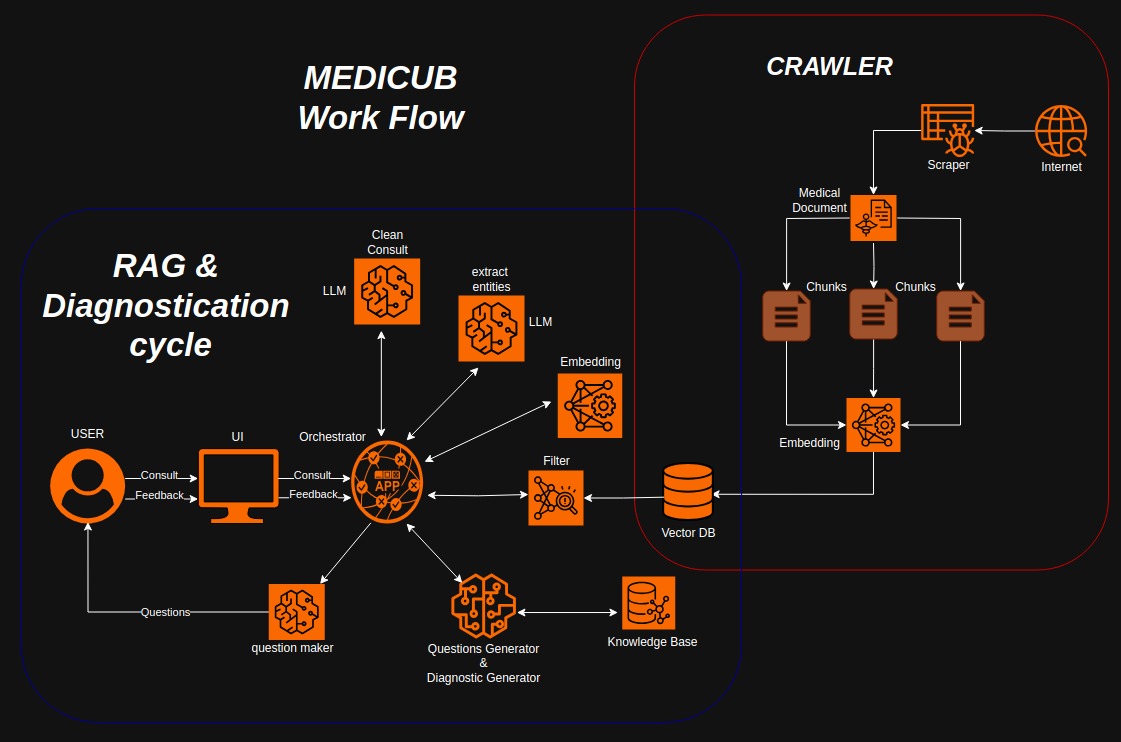
\includegraphics[scale=0.25]{Work Flow.png}
\end{center}
\caption{Flujo de trabajo del sistema}
\end{figure}

\section{Conclusiones}

La implementación del sistema MediCub ha permitido alcanzar importantes logros en la simulación del razonamiento clínico mediante inteligencia artificial. Se logró diseñar una arquitectura modular capaz de procesar consultas en lenguaje natural, extraer entidades médicas relevantes
y generar prediagnósticos fundamentados, incorporando un mecanismo de retroalimentación iterativa. Además, se integró una base de conocimientos médica actualizada automáticamente a partir de fuentes confiables lo que proporciona una sólida referencia para la toma de decisiones.

No obstante, se identifican varias limitaciones que condicionan la efectivadad del sistema. En primer lugar, la calidad de las respuestas generadadas depende de la claridad y precisión de la entrada proporcionada por el usuario, lo cual puede limitar la utilidad del sistema en escenarios
donde el paciente no pueda expresar sus síntomas de forma técnica o estructurada.

%
% ---- Bibliography ----
%
\begin{thebibliography}{5}
%
\bibitem {medlineplus}
MedlinePlus. (s.f.). \textit{Biblioteca Nacional de Medicina de EE.UU en Español}. Disponible en
\url{https://medlineplus.gov/spanish/}.

\bibitem{simulacion}
García Garrido, L., Martí Orosa, L., Pérez Sánchez, L.: \textit{Temas de Simulación}. Facultad de Matemática y Computación, Universidad de La Habana (s.f.)

\bibitem{fireworks_ai}
Fireworks.ai. (2025). \textit{Fireworks.ai}. Disponible en: \url{https://fireworks.ai/}.

\bibitem{fisterra}
Fisterra (2025). \textit{Información clínica para profesionales de la salud}. Dispnible en \url{https://www.fisterra.com/}.

\end{thebibliography}

\end{document}